\documentclass[9pt,a4paper,oneside,hidelinks,aspectratio=169,dvipsnames]{beamer}
\usepackage[outputdir=build]{minted}
\usepackage[T1]{fontenc}
\usepackage[utf8]{inputenc}
\usepackage[english]{babel}
\usepackage{datetime}
\usepackage{lmodern}
\usepackage{graphicx}
\usepackage{csquotes}
\usepackage{amsmath}
\usepackage{caption}
\usepackage{subcaption}
\usepackage{pifont}
\usepackage{xspace}
\usepackage{pgfplots}
\usepackage{tikz}

\usetheme[progressbar=frametitle]{metropolis}
\setbeamertemplate{section in toc}[sections numbered]
\captionsetup[figure]{font=tiny,labelsep=none}
\newcommand{\cmark}{\ding{51}\xspace}%
\newcommand{\xmark}{\ding{55}\xspace}%
\usetikzlibrary{automata, arrows.meta, shapes.geometric, calc, positioning, fit}

\title{Accelerating Halide on an FPGA by using CIRCT and Calyx as an intermediate step to go from a high-level and software-centric IRs down to RTL}
\date{May 15, 2023}
\author{Sergi Granell Escalfet}
\institute[Facultat d’Informàtica de Barcelona] {
  Master Degree in Innovation and Research in Informatics - High Performance Computing \\
  Facultat d’Informàtica de Barcelona \\
  Universitat Politècnica de Catalunya - BarcelonaTech
}

\pgfdeclareimage[height=0.6cm]{university-logo}{img/logo-upc-fib.png}
\logo{\pgfputat{\pgfxy(-1.4,-1.0)}{\pgfbox[center,base]{\pgfuseimage{university-logo}}}}

\begin{document}

\maketitle

\begin{frame}
  \frametitle{Table of Contents}
  \tableofcontents
\end{frame}

\section{Introduction}

\begin{frame}{Image and array processing}
  \begin{itemize}
    \item Image processing and array processing play an essential role in modern life:
          \begin{itemize}
            \item Applying filters to the images that we upload to social media
            \item Running object detection algorithms on self-driving cars
          \end{itemize}
    \item $\uparrow$ \textbf{Sophistication} modern image processing pipelines, resolution image sensors, real-time video processing $\implies$ $\uparrow$ demand for highly \textbf{efficient} image processing pipeline implementations
    \item \textbf{Diversity} of targets: from a small device such as a smartphone, smartwatch or edge device to large data center and HPC systems
    \item Optimizing these algorithms can be \textbf{complex} and often results in \textbf{non-portable code}
          \begin{itemize}
            \item Hand-tuned C and assembly for a specific architecture
            \item Implementations optimized for an x86 multicore and a modern GPU have little resemblance
          \end{itemize}
  \end{itemize}
\end{frame}

\begin{frame}{Domain Specific Languages (DSLs)}
  \begin{itemize}
    \item DSLs: programming languages specialized to a \textbf{particular application domain}
    \item \textbf{Abstraction}: they provide a higher level of abstraction tailored to the specific domain
          \begin{itemize}
            \item Making it easier for developers to express complex concepts and ideas in a concise and natural way
          \end{itemize}
    \item \textbf{Expressiveness}: by focusing on a specific domain, DSLs enable developers to express their intent more directly, resulting in more readable and maintainable code
    \item \textbf{Productivity}: they simplify the development process. Focus on solving domain-specific problems rather than low-level implementation details
    \item \textbf{Performance}: they can be optimized for the specific domain, potentially allowing more efficient execution and better performance
    \item For the image/array processing application domain $\implies$ \textbf{Halide}
  \end{itemize}
\end{frame}

\section{Halide}

\begin{frame}[fragile]{Halide}
  \begin{itemize}
    \item Main idea: \textbf{decouple} the \textcolor{blue}{\textbf{\textit{algorithm}}} (\textquote{what needs to be computed}) definition from its \textcolor{blue}{\textbf{\textit{schedule}}} (\textquote{how it should be computed})
    \item W/o changing algorithm, explore different optimizations strategies (loop nesting and loop fusion, tiling, recomputation and storage balancing, vectorization, parallelism, \ldots)
  \end{itemize}
  \begin{figure}[H]
    \centering
    \begin{minipage}{\textwidth}
      \centering
      \begin{subfigure}[H]{.4\textwidth}
        \inputminted[tabsize=2,frame=single,rulecolor=gray,fontsize=\fontsize{4.2}{3}]{cpp}{fig/halide_manual_opt.cpp}
        \caption*{Hand-optimized C\texttt{++}. $x11$ faster. 0.9 ms/megapixel.}
      \end{subfigure}
      $\implies$
      \begin{subfigure}[H]{.4\textwidth}
        \inputminted[escapeinside=||,tabsize=2,frame=single,rulecolor=gray,fontsize=\fontsize{4.2}{3}]{cpp}{fig/halide_blur_3x3.cpp}
        \caption*{0.9 ms/megapixel.}
      \end{subfigure}
    \end{minipage}
  \end{figure}
\end{frame}

\begin{frame}[fragile]{Scheduling trade-offs}
  \fontsize{6pt}{7.2}\selectfont
  \begin{figure}[H]
    \centering
    \begin{minipage}{0.325\textwidth}
      \inputminted[tabsize=2,frame=single,rulecolor=gray,fontsize=\fontsize{5}{5}]{cpp}{fig/blur_3x3_base.cpp}
      \caption*{Blur 3x3 filter algorithm}
    \end{minipage}
  \end{figure}
  \vspace{-0.5cm}
  \begin{figure}[H]
    \makebox[\linewidth]{
      \begin{minipage}{1.2\textwidth}
        \centering
        \begin{subfigure}[H]{.275\textwidth}
          \inputminted[tabsize=2,frame=single,rulecolor=gray,fontsize=\fontsize{4.2}{3}]{cpp}{fig/blur_3x3_breadth_first.cpp}
          \centering
          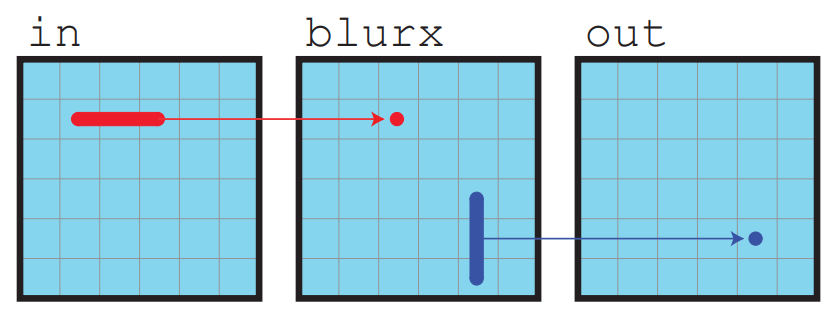
\includegraphics[width=3cm]{img/halide-breadth-first.png}
          \begin{itemize}
            \item[\xmark] Producer-consumer locality
            \item[\cmark] Parallelization
            \item[\cmark] Recomputation
          \end{itemize}
        \end{subfigure}
        \begin{subfigure}[H]{.31\textwidth}
          \inputminted[tabsize=2,frame=single,rulecolor=gray,fontsize=\fontsize{4.2}{3}]{cpp}{fig/blur_3x3_total_fusion.cpp}
          \vspace{0.3cm}
          \centering
          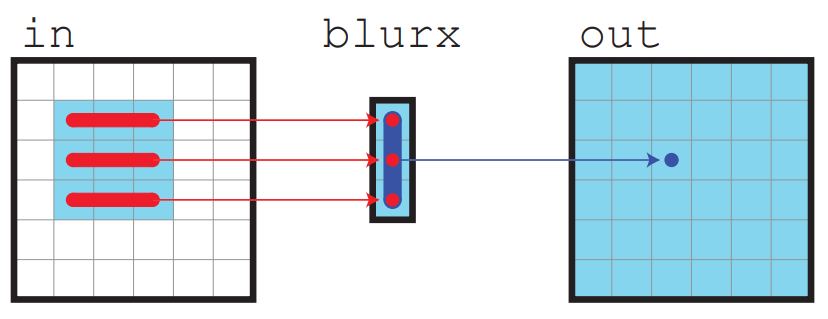
\includegraphics[width=3cm]{img/halide-total-fusion.png}
          \begin{itemize}
            \item[\cmark] Producer-consumer locality
            \item[\cmark] Parallelization
            \item[\xmark] Recomputation
          \end{itemize}
        \end{subfigure}
        \begin{subfigure}[H]{.3475\textwidth}
          \inputminted[tabsize=2,frame=single,rulecolor=gray,fontsize=\fontsize{4.2}{3}]{cpp}{fig/blur_3x3_sliding_window.cpp}
          \centering
          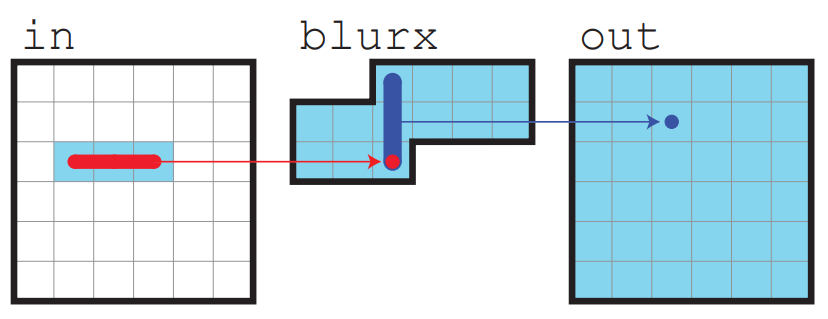
\includegraphics[width=3cm]{img/halide-sliding-window.png}
          \begin{itemize}
            \item[\cmark] Producer-consumer locality
            \item[\xmark] Parallelization
            \item[\cmark] Recomputation
          \end{itemize}
        \end{subfigure}
      \end{minipage}
    }
    \centering
    \unskip
    \vspace{0.5cm}
    \begin{tikzpicture}
      \coordinate (a) at (0cm,0cm);
      \coordinate (b) at (1.5cm,0);
      \coordinate (c) at (60:1.5cm);
      %
      \draw[color=black, fill=gray!40] (a) -- (b) -- (c) -- cycle;
      %
      \node[right = 0.1cm of b] {redundant work};
      \node[left = 0.1cm of a] {locality};
      \node[above = 0.1cm of c] {parallelism};
      \node[align=center] at (0.75cm, 0.4cm) {\tiny tradeoff\\\tiny space};
    \end{tikzpicture}
  \end{figure}
\end{frame}

\end{document}
